\section{Object-oriented Analysis}
\label{an:sec:analysis}

\subsection{System Sequence Diagrams (SSDs)}
\label{an:sub:system_sequence_diagrams}

\begin{itemize}
	\item Visualisierung von Interaktionen, welche die \textbf{Systemgrenze überschreiten}
	\item Basiert auf \textbf{simplifiziertem UML}
	\item Nähere Spezifizierung von \textbf{Reihenfolge}, \textbf{externen Events}, \textbf{Parametern und Return Values}
	\item Oftmals Beschränkung auf das \textbf{Main Success Scenario}, nutze \textbf{Use Cases} als Vorlage
\end{itemize}

\subsubsection{Beispiel}
\label{an:ssub:beispiel0}

\begin{figure}[!h]
	\centering
	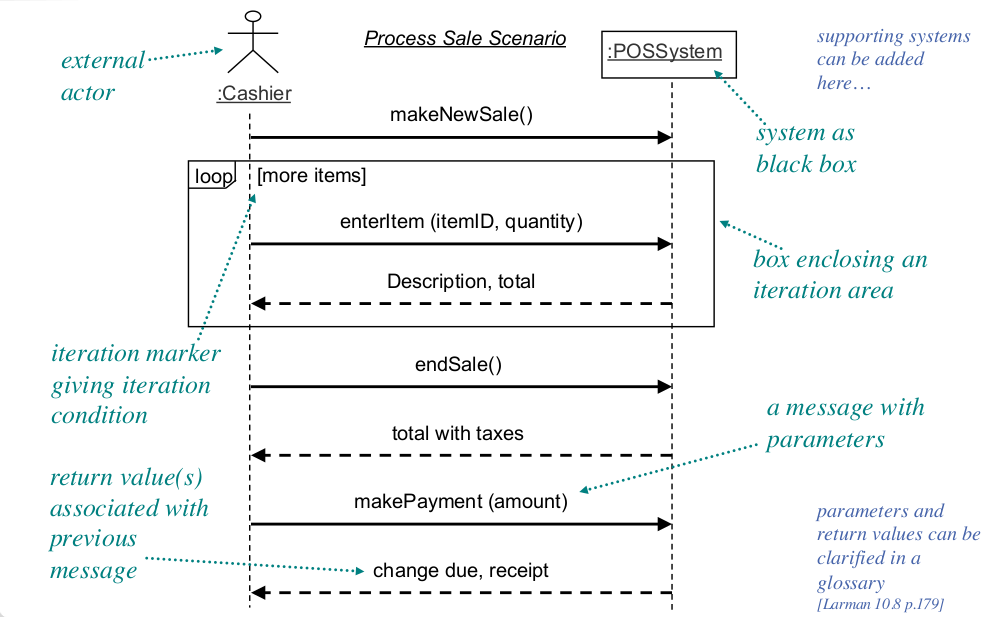
\includegraphics[width=0.85\textwidth]{images/ssd.png}
\end{figure}

\subsection{Domain Models}
\label{an:sub:domain_models}

\begin{itemize}
	\item Abstrakte Beschreibung der Entitäten innerhalb einer \textbf{Domain}, z.B mit UML
	\item Stoff aus SWT1, deshalb keine nähere Erklärung
	\item Neu: \textbf{Operation Contracts}
\end{itemize}

\subsubsection{Operation Contracts}
\label{an:ssub:operation_contracts}

\begin{itemize}
	\item Beschreibung, \textbf{was} für einen Zustandswechsel passieren muss
	\item Nähere Beschreibung der Operationen als in \textbf{Use Cases}, um letztere schlank zu halten
	\item Bei klaren Use Cases sind Contracts \textbf{optional}
	\item Benötigt zur Erstellung mindestens einen \textbf{Use Case}, nützlich zur Erstellung und Validierung von SSDs und Domain Models
	\item \textbf{Schema}:
	\begin{enumerate}
		\item \textbf{Operation}: Name, Parameter
		\item \textbf{Cross References}: optionale Auflistung der \textbf{Use Cases}, welche diese Operation referenzieren
		\item \textbf{Preconditions}: Wichtige Voraussetzungen, von deren Erfüllung ausgegangen wird
		\item \textbf{Postconditions}: Zustand des Domain Models nach der Operation
	\end{enumerate}
\end{itemize}

\subsubsection{Beispiel}
\label{an:ssub:beispiel1}

\begin{figure}[!h]
	\centering
	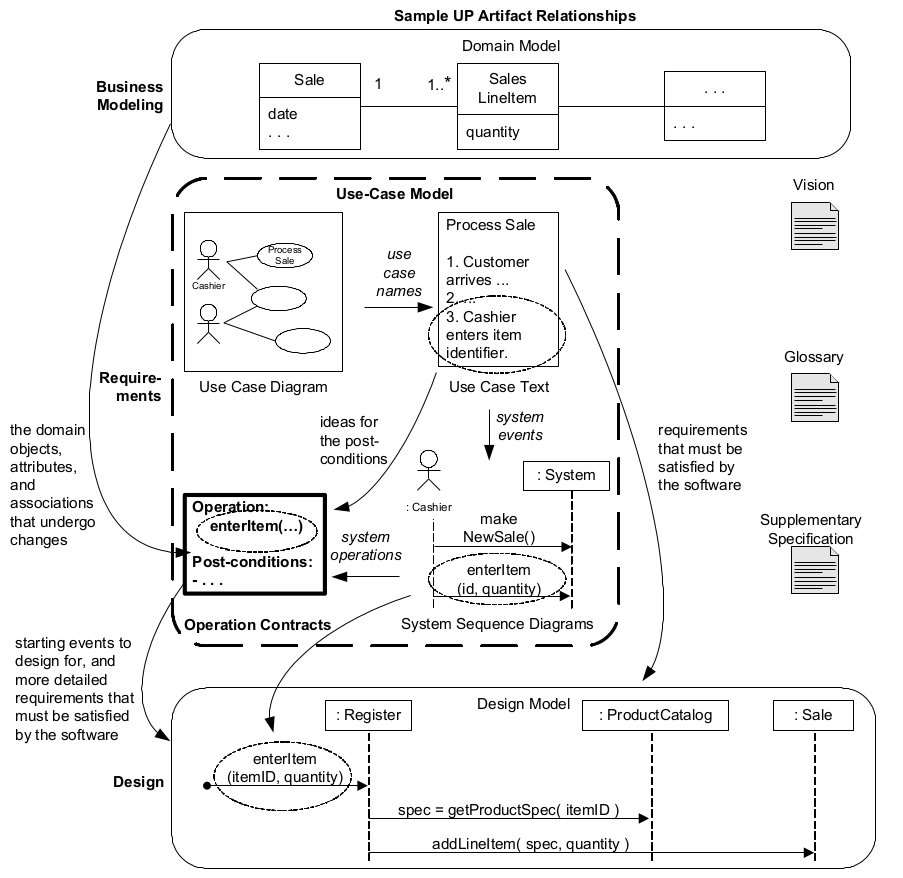
\includegraphics[width=0.85\textwidth]{images/domain_model.png}
\end{figure}